\section{Metodolog�a de desarrollo}
% Para el desarrollo de este proyecto se opto por la metodolog�a iterativa e incremental.
La metodolog�a de desarrollo es un conjunto de actividades relacionadas entre si y que se realizan en cierto orden definiendo un flujo de trabajo que permite llevar a cabo el desarrollo de un proyecto~\cite{Pressman2009}.

Una de estas metodolog�as es la iterativa e incremental. �sta metodolog�a, lleva a cabo el desarrollo de un proyecto de software dividi�ndolo en iteraciones que generan un incremento. Este incremento contribuye en el desarrollo del producto final~\cite{Alshamrani2015}.

Cada iteraci�n se compone de las fases de an�lisis, dise�o, implementaci�n y pruebas como se muestra en la Figura~\ref{fig:methodie}. La fase de an�lisis se encarga de llevar a cabo la obtenci�n y definici�n de los requerimientos del software. Durante la etapa de dise�o se realiza la conceptualizaci�n del software basado en los requerimientos definidos anteriormente. Durante la implementaci�n se codifican las funcionalidades siguiendo las directivas establecidas durante el dise�o, con el fin de satisfacer los requerimientos. Y finalmente, durante la fase de pruebas, se valida y verifica la correctitud de las funcionalidades implementadas, as� como el cumplimiento de los requisitos.

\begin{figure}[h]
	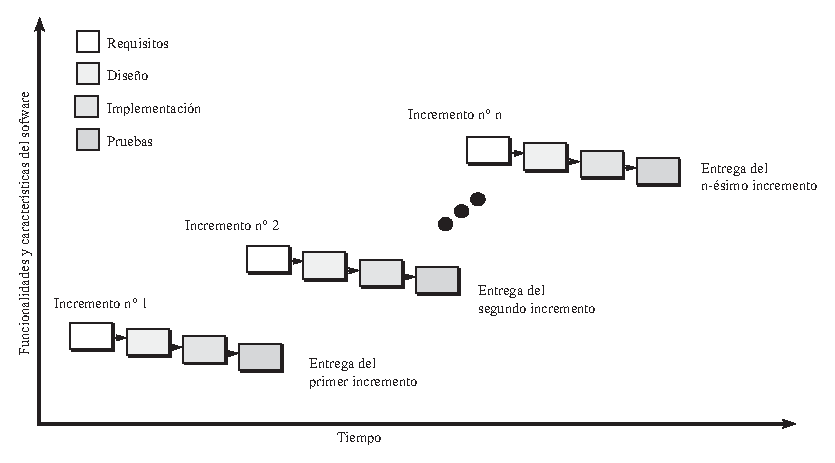
\includegraphics{Capitulo2/assets/iedevelopment-v2.eps}
	\centering
	\caption[Metodolog�a iterativa e incremental]{Metodolog�a iterativa e incremental~\cite{Pressman2009}}
	\label{fig:methodie}
\end{figure}

El hecho de llevar a cabo un desarrollo iterativo permite la obtenci�n de retroalimentaci�n del producto que se est� desarrollando y de esta manera poder refinar el trabajo en etapas posteriores del desarrollo~\cite{Victor2003, Mitchell2009, Martin1999,Alshamrani2015}.
